\let\negmedspace\undefined
\let\negthickspace\undefined
\documentclass[journal]{IEEEtran}
\usepackage[a5paper, margin=10mm, onecolumn]{geometry}
%\usepackage{lmodern} % Ensure lmodern is loaded for pdflatex
\usepackage{tfrupee} % Include tfrupee package

\setlength{\headheight}{1cm} % Set the height of the header box
\setlength{\headsep}{0mm}     % Set the distance between the header box and the top of the text

\usepackage{gvv-book}
\usepackage{gvv}
\usepackage{cite}
\usepackage{amsmath,amssymb,amsfonts,amsthm}
\usepackage{algorithmic}
\usepackage{graphicx}
\usepackage{textcomp}
\usepackage{xcolor}
\usepackage{txfonts}
\usepackage{listings}
\usepackage{enumitem}
\usepackage{mathtools}
\usepackage{gensymb}
\usepackage{comment}
\usepackage[breaklinks=true]{hyperref}
\usepackage{tkz-euclide} 
\usepackage{listings}
% \usepackage{gvv}                                        
\def\inputGnumericTable{}                                 
\usepackage[latin1]{inputenc}                                
\usepackage{color}                                            
\usepackage{array}                                            
\usepackage{longtable}                                       
\usepackage{calc}                                             
\usepackage{multirow}                                         
\usepackage{hhline}                                           
\usepackage{ifthen}                                           
\usepackage{lscape}
\begin{document}

\bibliographystyle{IEEEtran}
\vspace{3cm}

\title{AE - 2007}
\author{AI24BTECH11015 - Harshvardhan Patidar}
 \maketitle
% \newpage
% \bigskip
{\let\newpage\relax\maketitle}

\renewcommand{\thefigure}{\theenumi}
\renewcommand{\thetable}{\theenumi}
\setlength{\intextsep}{10pt} % Space between text and floats


\numberwithin{equation}{enumi}
\numberwithin{figure}{enumi}
\renewcommand{\thetable}{\theenumi}

\begin{enumerate}
	\item Shown in the figure \ref{25} below is a model of an Euler-Bernoulli beam made up of two materials subjected to pure bending moment $M$. The Young's modulus of material $A$ and $B$ are $E_A$ and $E_B$, respectively. The sectional moment of area, about the neutral axis, of the cross-sectional areas made of materials $A$ and $B$, are $I_A$ and $I_B$, respectively. The radius of curvature $\rho$ of the flexural deflection of this composite beam to the bending moment $M$ is then

		\begin{figure}[H]
			\centering
			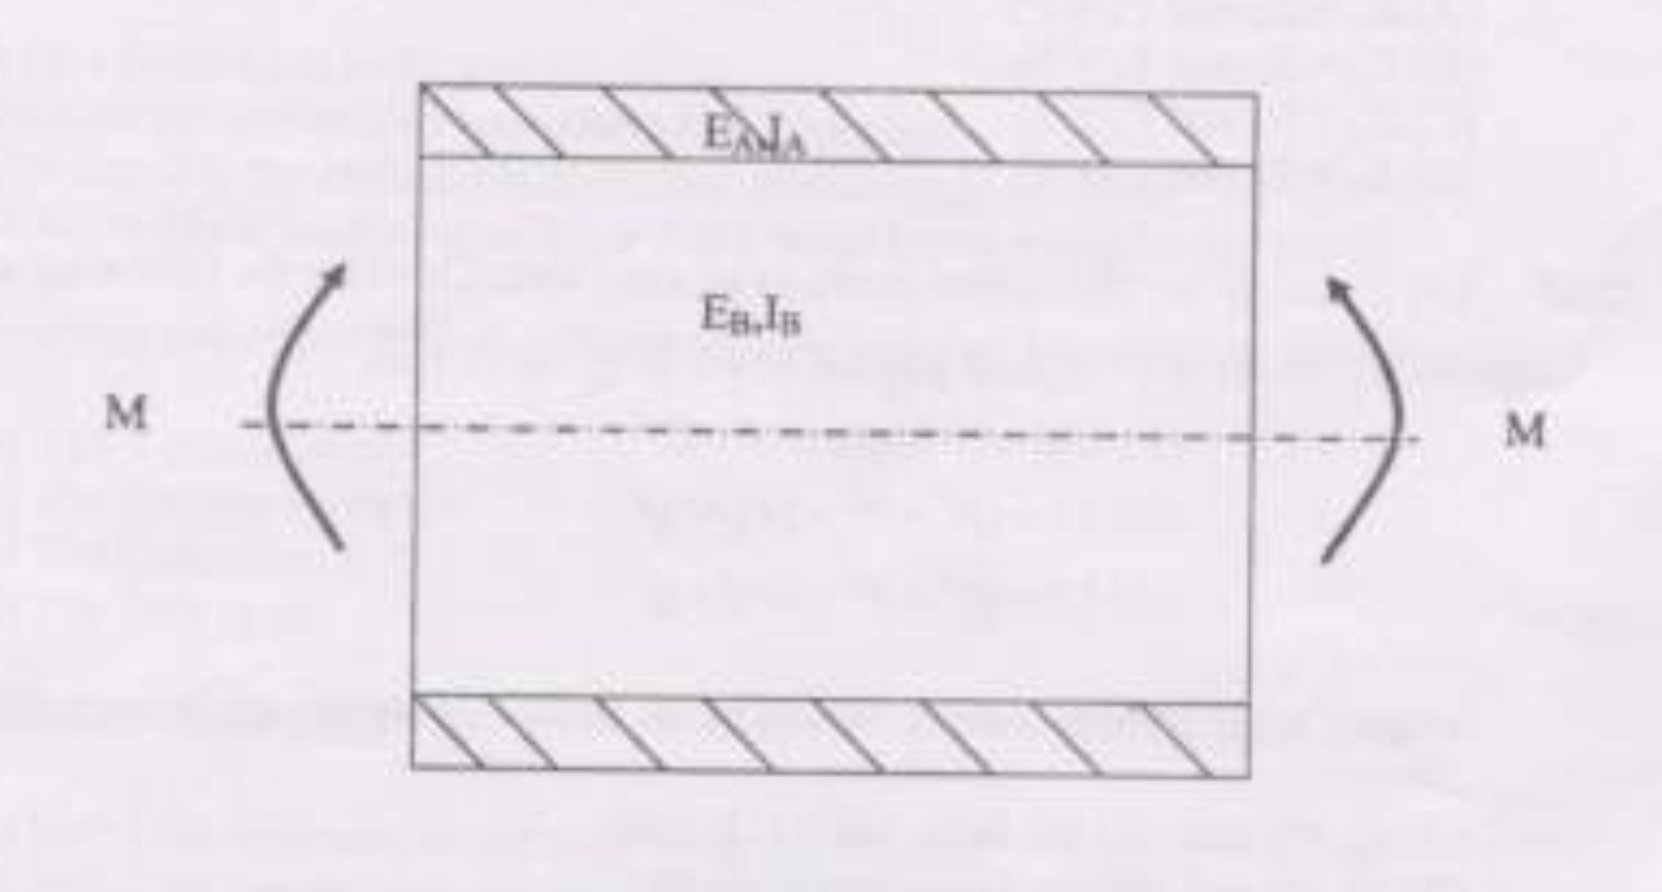
\includegraphics[width=\textwidth]{figs/25.png}
			\caption{}
			\label{25}
		\end{figure}


		\begin{enumerate}
    			\item $ \rho = \frac{E_A I_A + E_B I_B}{M} $
   			\item $ \rho = \frac{E_B I_A + E_A I_B}{M} $
  			\item $ \rho = \frac{M}{E_A I_A + E_B I_B} $
  			\item $ \rho = \frac{(E_A + E_B)(I_A + I_B)}{M} $
		\end{enumerate}


	\item Two pipes of constant sections but different diameters carry water at the same volume flow rate. The Reynolds number, based on the pipe diameter, is
		\begin{enumerate}
    			\item the same in both pipes
    			\item larger in the narrower pipe
    			\item smaller in the narrower pipe
    			\item depends on the material of the pipes
		\end{enumerate}

	\item 	Two airfoils of the same family are operating at the same angle of attack. The dimensions of one airfoil are twice as large as the other one. The ratio of the minimum pressure coefficient of the larger airfoil to the minimum pressure coefficient of the smaller airfoil is
		\begin{enumerate}
			\item $4.0$
    			\item $2.0$
    			\item $1.0$
    			\item $0.5$
		\end{enumerate}


	\item Wing A has a constant chord $c$ and span $b$. Wing B is identical but has a span $4b$. When both wings are opening at the same geometric angle of attack at subsonic speed, then:
		\begin{enumerate}
			\item wings A and B produce the same lift coefficient
			\item wing A produces a smaller lift coefficient than wing B
			\item wing A produces a greater lift coefficient than wing B
			\item the freestream Mach number decides which wing produces the greater lift coefficient
		\end{enumerate}


	\item A spring-mass-damper system is excited by a force $F_0 \sin \omega t$. The amplitude at resonance is measured to be $1cm$. At half the resonant frequency, the amplitude is $0.5cm$. The damping ratio of the system is
		\begin{enumerate}
			\item $0.1026$
			\item $0.3242$
			\item $0.7211$
			\item $0.1936$
		\end{enumerate}

	\item The eigenvalues of the matrix, $A = \myvec{2&1\\0&3}$. are
		\begin{enumerate}
			\item $1$ and $2$
			\item $1$ and $2$
			\item $2$ and $3$
			\item $2$ and $4$
		\end{enumerate}

	\item The eigenvalues of the matrix $A^{-1}$, where $A = \myvec{2&1\\0&3}$, are
		\begin{enumerate}
			\item $1$ and $\frac{1}{2}$
			\item $1$ and $\frac{1}{3}$
			\item $2$ and $3$
			\item $\frac{1}{2}$ and $\frac{1}{3}$
		\end{enumerate}

	\item The radius of the earth is $6.37 \times 10^4 m$ and the acceleration due to gravity at its surface is $9.81 m / s^2$. A satellite is in circular orbit at a height of $35.9\times 10^6 m$ above the earth's surface. This orbit is inclined at $10.5$ degrees to the equator. The velocity change needed to make the orbit equatorial is:
		\begin{enumerate}
			\item $561 m / s$ at $84.75$ degrees to the initial direction
			\item $561 m / s$ at $95.25$ degrees to the initial direction
			\item $281 m / s$ at $84.75$ degrees to the initial direction
			\item $281 m / s$ at $95.25$ degrees to the initial direction
		\end{enumerate}

	\item A piston-prop airplane having propeller efficiency, $\eta_p = 0.8$ and weighing $73108 N$ could achieve maximum climb rate of $15m/s$ at flight speed of $50m/s$. The excess Brake Power \brak{BP} at the above flight condition will be
		\begin{enumerate}
			\item $1700$ kW
			\item $2100$ kW
			\item $1371$ kW
			\item $6125$ kW
		\end{enumerate}
	\item An airplane model with a symmetric airfoil was tested in a wind tunnel $C_{m,0}$ ($C_m$ at angle of attack, $\alpha = 0$) was estimated to be $0.08$ and $0$ respectively for elevator settings ($\delta _ e$) of $5$ degrees up and $5$ degrees down. The estimated value of the elevator control power $\brak{\frac{\partial C_m}{\partial \delta _ e}}$ of the model will be 
		\begin{enumerate}
			\item $0.07$ per deg
			\item $-1.065$ per deg
			\item $-0.008$ per deg
			\item $-0.762$ per deg
		\end{enumerate}

	\item The lateral-directional characteristic equation for an airplane gave the following set of roots: $\lambda _ 1 = -0.6, \lambda _ 2 = -0.002, \lambda _{3,4} = -0.06 \pm f1.5$, where $f = \sqrt{-1}$. The damping ratio corresponding to the Dutch-roll mode will be
		\begin{enumerate}
			\item $0.04$
			\item $0.66$
			\item $0.35$
			\item $0.18$
		\end{enumerate}

	\item An airplane is flying at an altitude of $10km$ above the sea level. Outside air temperature and density at $10km$ altitude are $223 K$ and $0.413 kg/ m^3 $ respectively. The airspeed indicator of the airplane indicates a speed of $60 m/s$. Density of air at sea level is $1.225 kg/m^3$ and value of the gas constant $R$ is $288 J/kg/K$. The stagnation pressure $\brak{P_e}$ measured by the Pitot tube mounted on the wing tip of the airplane will be of magnitude
		\begin{enumerate}
			\item $3.5 \times 10^4 N/m^2$
			\item $2.0 \times 10^4 N/m^2$
			\item $2.87 \times 10^4 N/m^2$
			\item $0.6 \times 10^4 N/m^2$
		\end{enumerate}

	\item If the center of gravity of an airplane is moved forward towards the nose of the airplane, the $C_{L max}$(maximum value fo the lift coefficient) value for which the airplane can be trimmed $\brak{C_m = 0}$ will
		\begin{enumerate}
			\item decrease
			\item increase
			\item remain same
			\item depend upon rudder deflection
		\end{enumerate}

	\item If the contribution of only the horizontal tail of an airplane was considered for estimating $\frac{\partial C_m}{\partial \alpha}$, and if the tail moment arm $l$, was doubled, then how many times the original value would the new $\frac{\partial C_m}{\partial \alpha}$ become ?
		\begin{enumerate}
			\item two times
			\item three times
			\item $1.414$ times
			\item $1.732$ times
		\end{enumerate}

	\item If the vertical tail of an airplane is inverted and put below the horizontal tail, then the contribution to roll derivative, $\frac{\partial C_I}{\partial \beta}$, will be
		\begin{enumerate}
			\item negative
			\item positive
			\item zero
			\item imaginary
		\end{enumerate}
		
		
	\item Let a system of linear equations be as follows:
		\begin{align*}
			x - y + 2z &= 0\\
			2x + 3y - z &= 0\\
			2x-2y+4z &=0
		\end{align*}
		This system of equations has

		\begin{enumerate}
			\item No non-trivial solution
			\item Infinite number of non-trivial solutions
			\item An unique non-trivial solution
			\item Two non-trivial solutions
		\end{enumerate}

	\item A turbulent boundary layer remains attached over a longer distance on the upper surface of an airfoil than does a laminar boundary layer, because
		\begin{enumerate}
			\item the turbulent boundary layer is more energetic and hence can overcome the adverse pressure gradient better
			\item the laminar boundary layer develops more skin friction and hence slows down more rapidly
			\item turbulence causes the effective coefficient of viscosity to reduce, resulting in less loss of momentum in the bounday layer
			\item the turbulent boundary layer is thicker, hence the velocity gradients in it are smaller, therefore viscous losses are less
		\end{enumerate}

\end{enumerate}

  
\end{document}


